\documentclass[tikz,border=10pt]{standalone}
\usepackage{mathtools}
\usepackage{amssymb}

\begin{document}

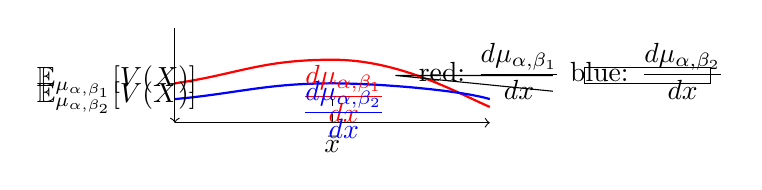
\begin{tikzpicture}[xscale=4]
    % Axes
    \draw[->] (0,1.2) -- (0,0) node[below left] {} ;
    \draw[->] (0,0) -- (1,0) node[below right] {} ;
    % Curves
    \draw[red, thick] (0,0.5) to[out=30,in=180] (0.5,0.8) to[out=0,in=120,looseness=0.7] (1,0.2) ;
    \draw[blue, thick] (0,0.3) to[out=20,in=180] (0.5,0.5) to[out=0,in=130,looseness=0.7] (1,0.3) ;
    % Point
    \draw[dashed] (0.5,0) -- (0.5,0.3) ;
    \node[below] at (0.5,-0.05) {$\bar{x}$} ;
    % Legend
    \begin{scope}[shift={(0.7,0.5)}]
        \draw (0.5,0.1) -- (0,0.1) -- (0.5,-0.1) ;
        \draw (0.6,0) rectangle (1,0.2) ;
        \node at (0.3,0.15) {red: $\dfrac{d\mu_{\alpha,\beta_1}}{dx}$} ;
        \node at (0.8,0.15) {blue: $\dfrac{d\mu_{\alpha,\beta_2}}{dx}$} ;
    \end{scope}
    % Text
    \node[anchor=north east] at (0.1,0.85) {$\mathbb{E}_{\mu_{\alpha,\beta_1}}[V(X)]$};
    \node[anchor=north east] at (0.1,0.65) {$\mathbb{E}_{\mu_{\alpha,\beta_2}}[V(X)]$};
    \node[anchor=north east, red] at (0.7,0.85) {$\dfrac{d\mu_{\alpha,\beta_1}}{dx}$};
    \node[anchor=north east, blue] at (0.7,0.65) {$\dfrac{d\mu_{\alpha,\beta_2}}{dx}$};
\end{tikzpicture}

\end{document}